\documentclass[12px]{article}

\usepackage{tikz}
\usepackage{geometry}
\usetikzlibrary{mindmap}

\geometry{landscape, margin=1cm}

\begin{document}
\begin{center}
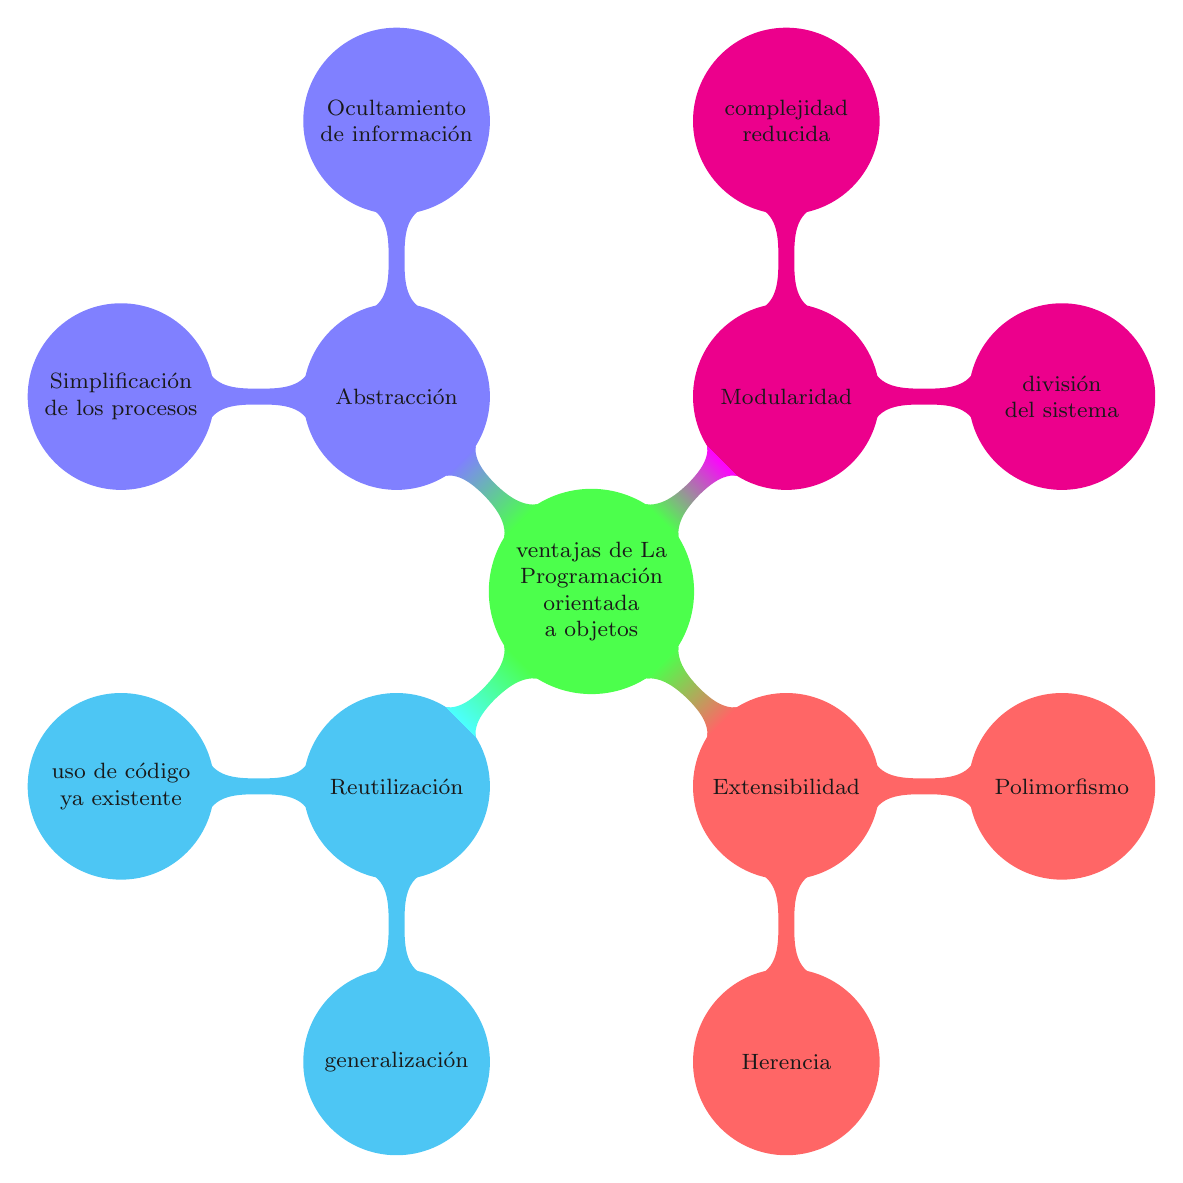
\begin{tikzpicture}[small mindmap, grow cyclic, every node/.style=concept, concept color=green!70, text=black!90,
    level 1/.style={level distance=3.5cm, sibling angle=360/4},
    level 2/.style={level distance=3.5cm, sibling angle=360/4}]
    \node {ventajas de La Programación orientada a objetos}
        child[concept color=cyan!70] { node {Reutilización}
            child { node { uso de código ya existente } }
            child { node { generalización } }
        }
        child[concept color=red!60] { node { Extensibilidad }
            child { node { Herencia } }
            child { node { Polimorfismo } }
        }
        child[concept color=magenta] { node { Modularidad }
            child { node { división del sistema } }
            child { node { complejidad reducida } }
        }
        child[concept color=blue!50] { node { Abstracción }
            child { node { Ocultamiento de información } }
            child { node { Simplificación de los procesos } }
        }
    ;
\end{tikzpicture}
\end{center}
\end{document}
